\documentclass[tikz,border=5pt]{standalone}
\usepackage{tikz}
\usetikzlibrary{arrows.meta,decorations.pathmorphing}

% Atlas color palette
\definecolor{AtlasTeal}{HTML}{5BA4A4}
\definecolor{AtlasWarm}{HTML}{C17F59}
\definecolor{AtlasSage}{HTML}{7A9E7E}

\begin{document}
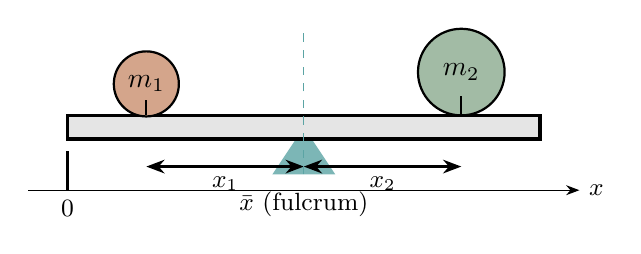
\begin{tikzpicture}[
    mass/.style={draw=black, thick, fill=#1, minimum size=0.8cm, circle},
    >=Stealth
]
    % Fulcrum (triangle)
    \fill[AtlasTeal!80] (3,0) -- (2.6,-0.6) -- (3.4,-0.6) -- cycle;
    
    % Beam (lever/seesaw)
    \draw[very thick, fill=gray!20] (0,0.15) rectangle (6,-0.15);
    
    % Mass 1 (left, smaller)
    \node[mass=AtlasWarm!70] at (1,0.55) {$m_1$};
    \draw[thick] (1,0.15) -- (1,0.35);
    
    % Mass 2 (right, larger)
    \node[mass=AtlasSage!70, minimum size=1.1cm] at (5,0.7) {$m_2$};
    \draw[thick] (5,0.15) -- (5,0.4);
    
    % Position markers
    \draw[<->, thick] (1,-0.5) -- node[below, font=\small] {$x_1$} (3,-0.5);
    \draw[<->, thick] (3,-0.5) -- node[below, font=\small] {$x_2$} (5,-0.5);
    
    % Fulcrum label
    \node[below, font=\small] at (3,-0.7) {$\bar{x}$ (fulcrum)};
    
    % Origin marker
    \draw[thick] (0,-0.8) -- (0,-0.3);
    \node[below, font=\small] at (0,-0.8) {$0$};
    
    % Axis
    \draw[->] (-0.5,-0.8) -- (6.5,-0.8) node[right, font=\small] {$x$};
    
    % Balance indication
    \draw[dashed, AtlasTeal] (3,-0.6) -- (3,1.2);
\end{tikzpicture}
\end{document}
